% 2002 年全国旧课程文科第 19 题：四棱锥 P-ABCD
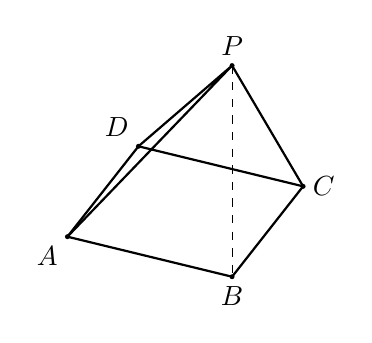
\begin{tikzpicture}[>=stealth,scale=0.82]
  \coordinate (A) at (0,0);
  \coordinate (B) at (2.55,-0.62);
  \coordinate (C) at (3.65,0.78);
  \coordinate (D) at (1.10,1.40);
  \coordinate (P) at (2.55,2.65);
  \draw[thick] (A)--(B)--(C)--(D)--cycle;
  \draw[thick] (P)--(A) (P)--(C) (P)--(D);
  \draw[dashed] (P)--(B);
  \fill (A) circle (1.1pt) node[below left] {$A$};
  \fill (B) circle (1.1pt) node[below] {$B$};
  \fill (C) circle (1.1pt) node[right] {$C$};
  \fill (D) circle (1.1pt) node[above left] {$D$};
  \fill (P) circle (1.1pt) node[above] {$P$};
\end{tikzpicture}
